% !TEX root = ../review.tex
% \begin{frame}
% \frametitle{OPTIMA: Общие сведения}


% \end{frame}

\begin{frame}
\frametitle{OPTIMA: Алгоритм}

Этапы выравнивания:
\begin{itemize}
  \item Поиск стартовых мест (сидов) для начала выравнивания
  \item Парное выравнивание карты с референсом
  \item Определение значимых выравниваний
  \item Объединение пересекающихся выравниваний
\end{itemize}

\end{frame}

\begin{frame}
\frametitle{OPTIMA: Композитные сиды}
Композитные сиды:
\begin{figure}
  \centering
  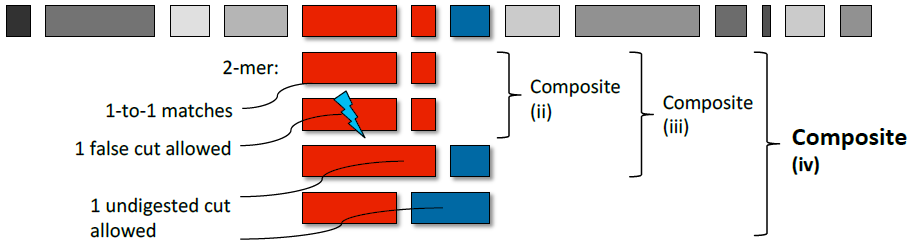
\includegraphics[width = 0.9\textwidth]{optima/composite_seeds}
\end{figure}
\textbf{Определение.} \\
Множество фрагментов $o_k$, $o_{k + 1}$, $ \dots$, $o_{s}$ \textbf{возможно
совпадает} с множеством фрагментов $r_l$, $r_{l+1}$, $\dots$, $r_{t}$ :
\begin{gather}
\frac{\bigg|\sum\limits_{i = k}^s o_i - \sum\limits_{j = l}^t r_j \bigg|}{\sqrt{\sum\limits_{j = l}^t \sigma_j^2}} \le C_{\sigma}
\label{eq:feasible_match}
\end{gather}
где $C_{\sigma}$ - порог совпадения, $\sigma_j$ - стандартное отклонение $r_j$

\end{frame}

\begin{frame}
\frametitle{OPTIMA: Поиск стартовых сидов}
Алгоритм поиска сидов для выравнивания:
\begin{itemize}
  \item По референсу строятся композитные сиды и сортируются по первому элементу
  \item У карты берётся сид, по которому будем искать множество подходящих локаций (\ref{eq:feasible_match}) в референсе
  \item Бинарным поиском (по первому элементу) ищем множество подходящих сидов в референсе
  \item Далее линейно проверяем и оставляем только те, которые удовлетворяют (\ref{eq:feasible_match})
  \item Таким образом получаем множество сидов на референсе, где карта может быть выравнена
  \item Сложность алгоритма $O(m \, (log \, n + k \, \#seeds_{k=1}))$\\
  $n$ и $m$ - количество фрагментов в референсе и карте \\
  $k$ - длина k-tuple \\
  $\#seeds_{k=1}$ - количество сидов найденных по первому элементу
\end{itemize}
\end{frame}

\begin{frame}
\frametitle{OPTIMA: Парное выравнивание карты с референсом}
После обнаружения схожих сидов на референсе происходит парное выравнивание алгоритмом динамического программирования:
\begin{gather*}
Score_{s,t} = \min\limits_{k \le s, l \le t} C_{ce} \, (s - k + t - l) + \chi_{k \dots s, l \dots t}^2 + Score_{k-1,l-1} \\
\chi_{k \dots s, l \dots t}^2 = \frac{\bigg(\sum\limits_{i = k}^s o_i - \sum\limits_{j = l}^t r_j \bigg)^2}{\sum\limits_{j = l}^t\sigma_j^2}
\end{gather*}
$C_{se}$ - штраф за пропущенные разрезы
\end{frame}

\begin{frame}
\frametitle{OPTIMA: Определение значимости выравнивания}
Пусть $a$ - выравнивание из множества выравниваний $\mathcal{A}$
\begin{gather*}
Z-score(a \in \mathcal{A}, f) = \frac{f_{a} - Mean(f_{\mathcal{A}})}{SD(f_{\mathcal{A}})}
\end{gather*}
где $f$ - характеристика выравнивания.\\
 Тогда статистическая значимость выравнивания:
\begin{align*}
  \vartheta (a \in \mathcal{A}) = Z-score( & -Z-score(a, \#matches) \\
  & + Z-score(a, \#cuterrors) \\
  & + Z-score(a, WHT(\chi^2, \#matches))) \\
\end{align*}
\[\text{где } WHT(\chi^2, \#matches) = \frac{\sqrt[3]{\frac{\chi^2}{\#matches}} - \big(1 - \frac{1}{9} \frac{2}{\#matches}\big)}{\sqrt{\frac{1}{9} \frac{2}{\#matches}}}\]
\end{frame}

\begin{frame}
\frametitle{OPTIMA: Пример множества выравниваний}
\begin{figure}
  \centering
  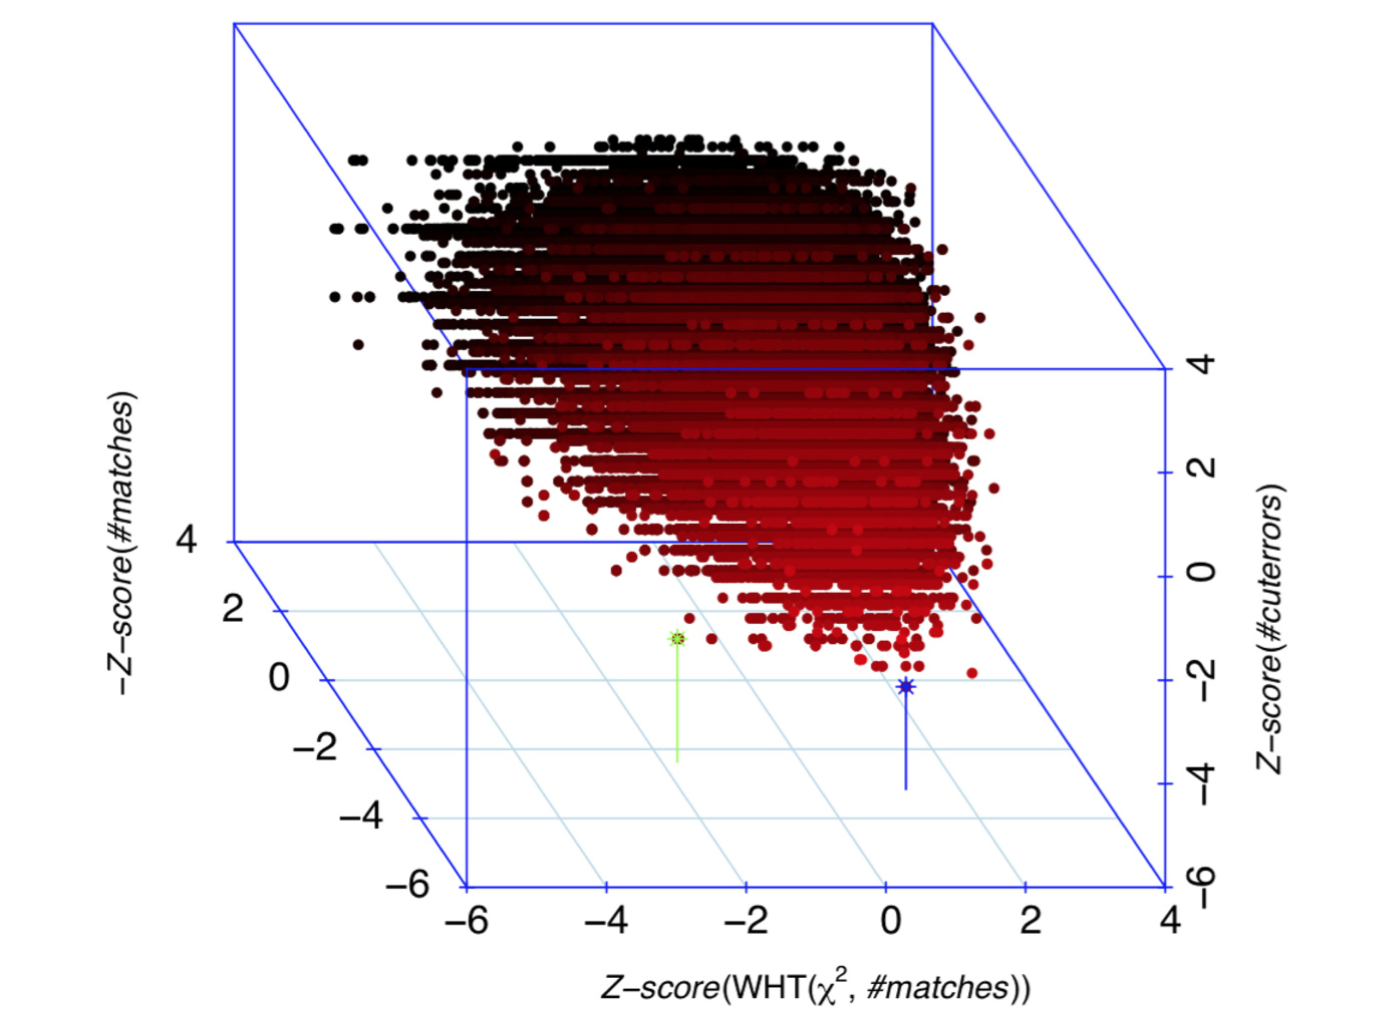
\includegraphics[width = 0.9\textwidth]{optima/cube}
\end{figure}
\end{frame}


% \begin{frame}
% \frametitle{OPTIMA: Объединение пересекающихся выравниваний}
% Разбиение на блоки:
% \begin{figure}
%   \centering
%   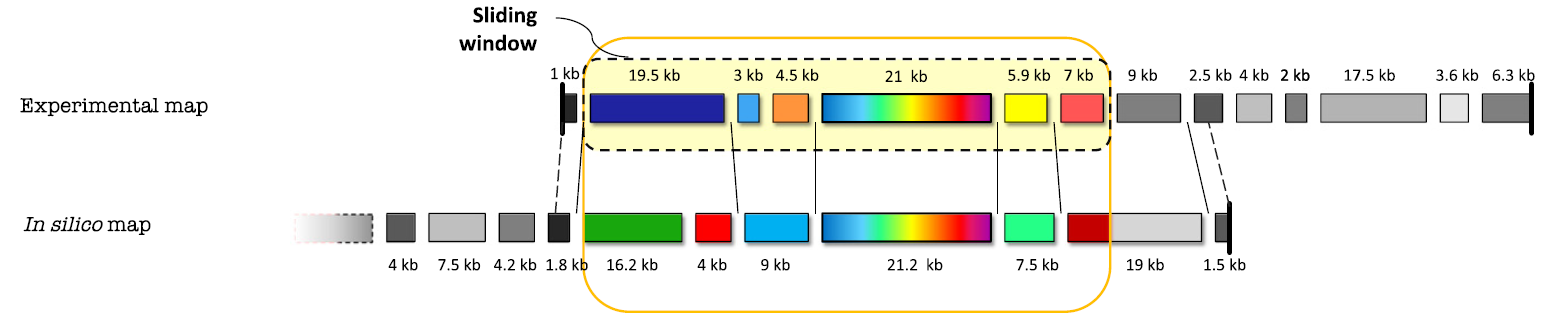
\includegraphics[width = 0.9\textwidth]{optima/extension}
% \end{figure}
% \end{frame}

\begin{frame}
\frametitle{OPTIMA: Результаты}
Результаты для 2100 карт:
\begin{figure}
  \centering
  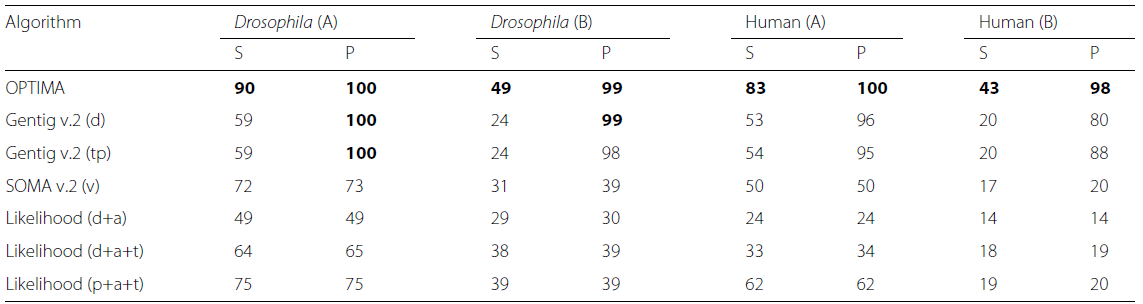
\includegraphics[width = 0.9\textwidth]{optima/results}
\end{figure}
S - чувствительность \\
P - точность \\
tp - настройка параметров в соответствии с генерацией данных \\
p - параметры, указанные в статьях авторов \\
d - стандартные настройки \\
t - обрезание концов карт \\
a - скорректированные на основе анализа организма
\end{frame}

\begin{frame}
\frametitle{OPTIMA: Время работы}
Ожидаемое время работы:
\begin{figure}
  \centering
  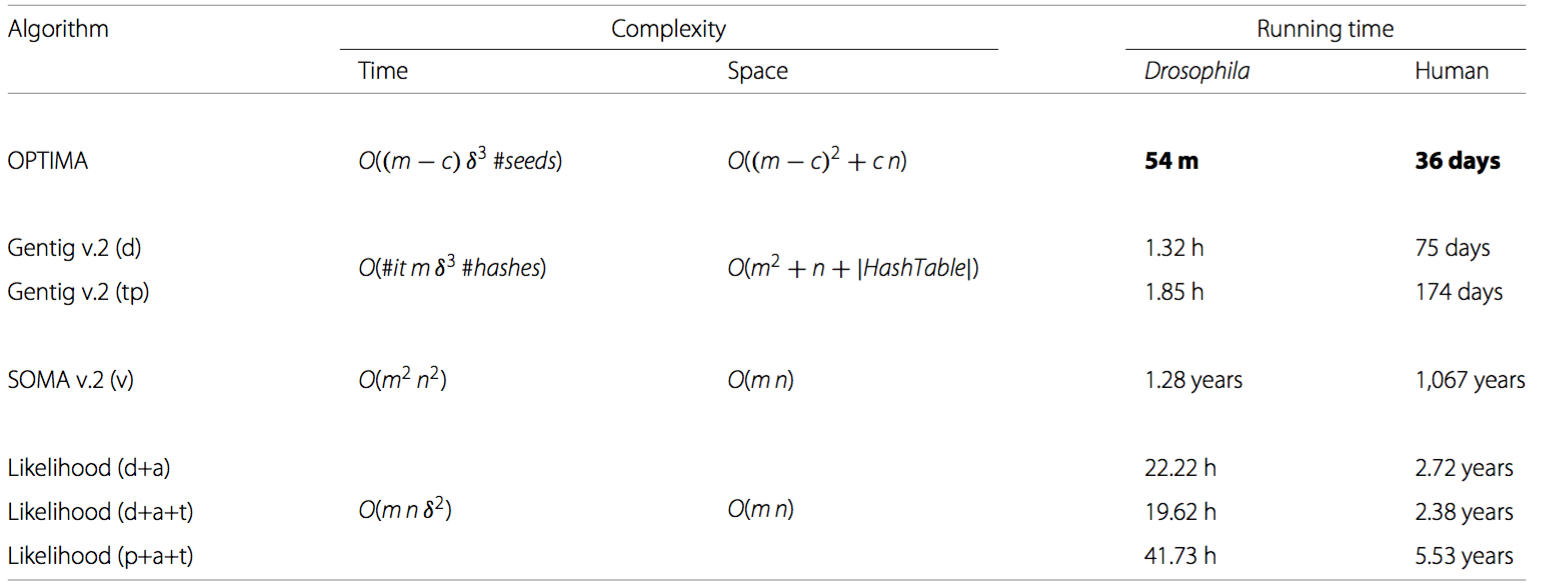
\includegraphics[width = 0.9\textwidth]{optima/time}
\end{figure}
Drosophila - 82000 карт \\
Human - 2100000 карт
\end{frame}
